\subsection{Video Collection and Outlier Detection}
\label{filter}
As we explain in the Section~\ref{sec:overview}, our system starts with querying the YouTube for the recipe which we want to learn its fine-grained actions. Although we explain how do we choose such queries in Section~\ref{dataset:sec} detail, any query starting with \emph{How to} can be considered as an example. We collect the top 100 videos with their (automatically generated) captions. YouTube generates these captions by using an Automatic Speech Recognition (ASR) algorithm. After obtaining the corpus, we link similar videos to each other by creating a kNN video graph. As a distance metric, we use the bag-of-words model of video descriptions. We compute the bag-of-words representation of each description and use $\chi^2$-distance of them as a distance metric. After the creation of the graph, we compute the dominant cluster by using the Single Cluster Graph Partitioning (SCGP)\cite{scgp} discards the remaining videos as outlier.

As an example, in Figure~\ref{outliers} we visualize some of the discarded videos for the query \emph{How to make a milkshake?}. As shown in the figure, they are actual outliers like making a toy milkshake, making a milkshake charm and a funny video about How to NOT make milkshakes.
\begin{figure}[ht]
  \begin{subfigure}[b]{0.16\textwidth}
    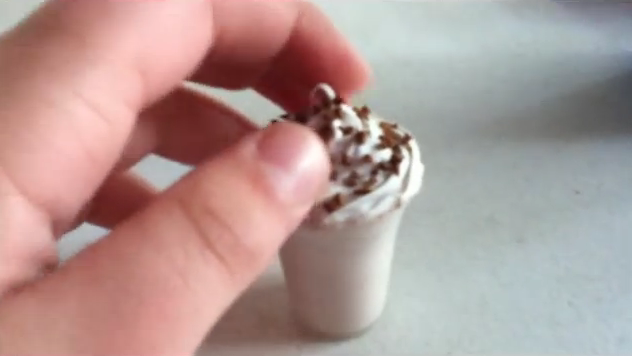
\includegraphics[width=\textwidth]{troll_1}
  \end{subfigure}~
  \begin{subfigure}[b]{0.16\textwidth}
    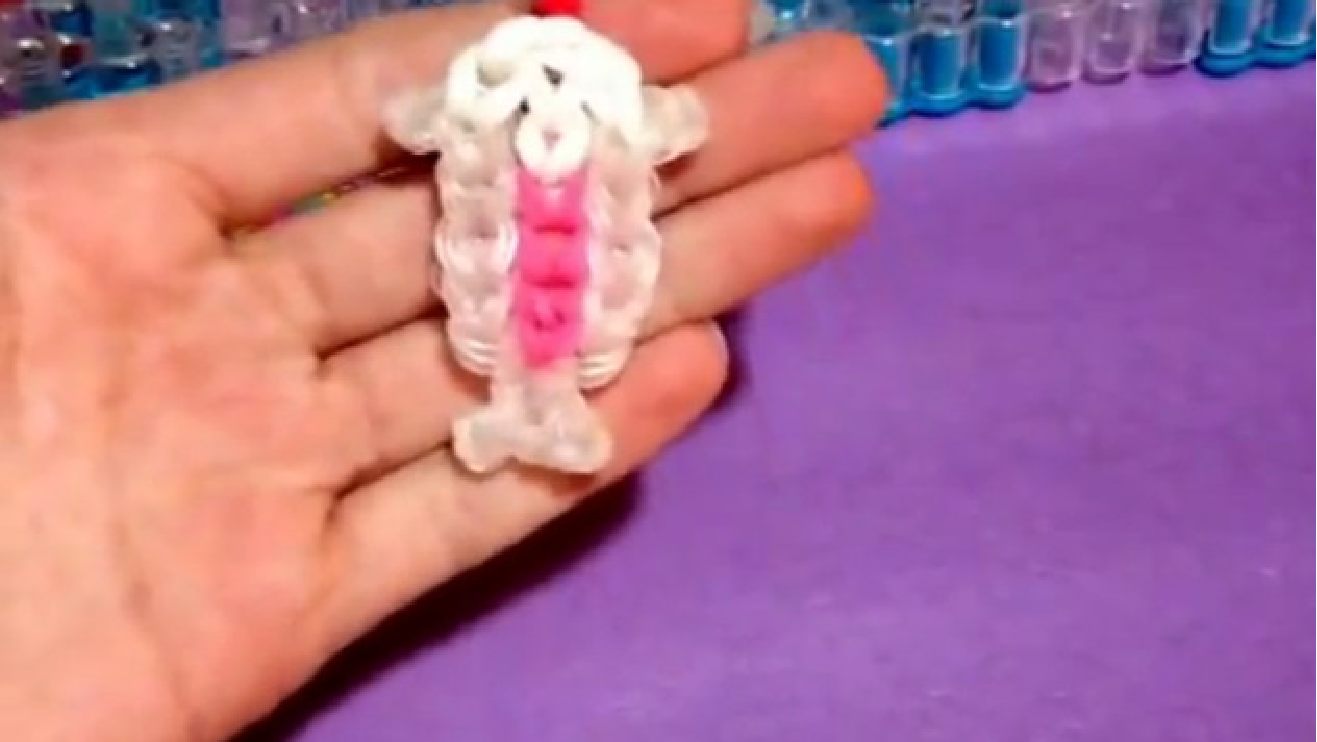
\includegraphics[width=\textwidth]{troll_2}
  \end{subfigure}~
  \begin{subfigure}[b]{0.16\textwidth}
    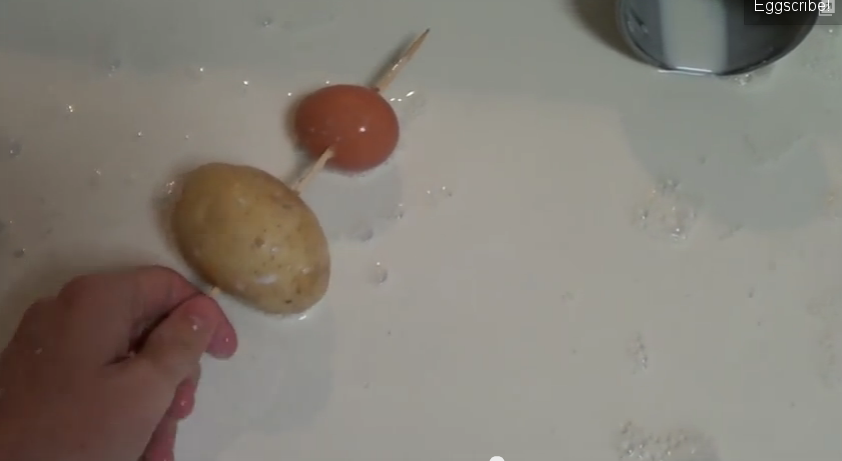
\includegraphics[width=\textwidth]{troll_3}
  \end{subfigure}
\caption{\textbf{Sample videos which our algorithm discards as an outlier for the query \emph{How to make a milkshake?}.} These videos are about a toy milkshake, a milkshake charm and a funny video about How to NOT make milkshakes.}
\label{outliers}
\end{figure}

\subsection{Semantic Multi-Modal Frame Representation}
We represent the each frame of the each video by using set of language and visual atoms which we automatically extract. Language atoms are the salient words learned by ranking the words in the subtitle corpus via tf-idf like measure. And, the visual atoms are found by clustering over region proposals which we extract from each frame. We explain the details of proposal generation, clustering and ranking in the subsequent sections.

\subsubsection{Learning Language Atoms}
After obtaining the videos and subtitles belonging to a single query, we concatenate all subtitles into a single collection(term corpus). As a document, we use all the words extracted from all subtitles of all queries. Moreover, we compute the tf-idf as $tfidf(w,d,D)=f_{w,d} \times \log \frac{N}{n_{w}}$ where $w$ is the word, $d$ is the collection of words corresponding to the query, $f_{w,d}$ is the frequency of the word in the collection $d$, $N$ is the total number of videos returned from all queries and $n_{w}$ is the number of videos whose subtitle include the word $w$. After computing the tf-idf, we sort all words with their tf-idf values and choose the top $K$ words as set of salient words (\emph{We set $K=100$ in our experiments}).

We show below the top 50 salient words extracted for the query \emph{How to hard boil an egg?}. Moreover, they correspond to important objects, actions and adjectives which can semantically relate actions over multiple videos.

\footnotesize
\emph{sort, place, water, egg, bottom, fresh, pot, crack, cold, cover, time, overcooking, hot, shell, stove, turn, cook, boil, break, pinch, salt, peel, lid, point, high, rules, perfectly, hard, smell, fast, soft, chill, ice, bowl, remove, aside, store, set, temperature, coagulates, yolk, drain, swirl, shake, white, roll, handle, surface, flat}
\normalsize


\subsubsection{Learning Visual Atoms}
In order to learn visual atoms, we create a large collection of proposals by independently generating region proposals from each frame of the each video. These proposals are generated by using the Constrained Parametric Min-Cut (CPMC) \cite{cpmc} algorithm by using both appearance and motion cues. We note the $k^{th}$ region of $t^{th}$ frame of $i^{th}$ video as $r^{(i),k}_t$. Moreover, we drop the video index $(i)$ if it is clear from the context.

We follow the spectral graph clustering approach in order to group these regions into semantically meaningful objects similar to the Keysegments approach \cite{keysegments}. However, idea of clustering region proposals into set of semantic objects have been mostly utilized for clusters generated by a single video and they fail to cluster objects having a large visual difference. Hence, we extend this work to spectral joint clustering of region proposals over multiple videos.

\paragraph{Joint Proposal Clustering to Detect Visual Objects}
Since our proposals are generated from multiple videos, combining them into a single region collection and clustering it is not desired for two reasons; (1) objects have large visual differences among videos and accurately clustering them into a single cluster is hard, (2) clusters are desired to have region proposals from multiple videos in order to semantically relate videos. We propose a joint version of the spectral region clustering algorithm to satisfy these requirements.

\begin{figure}[ht]
  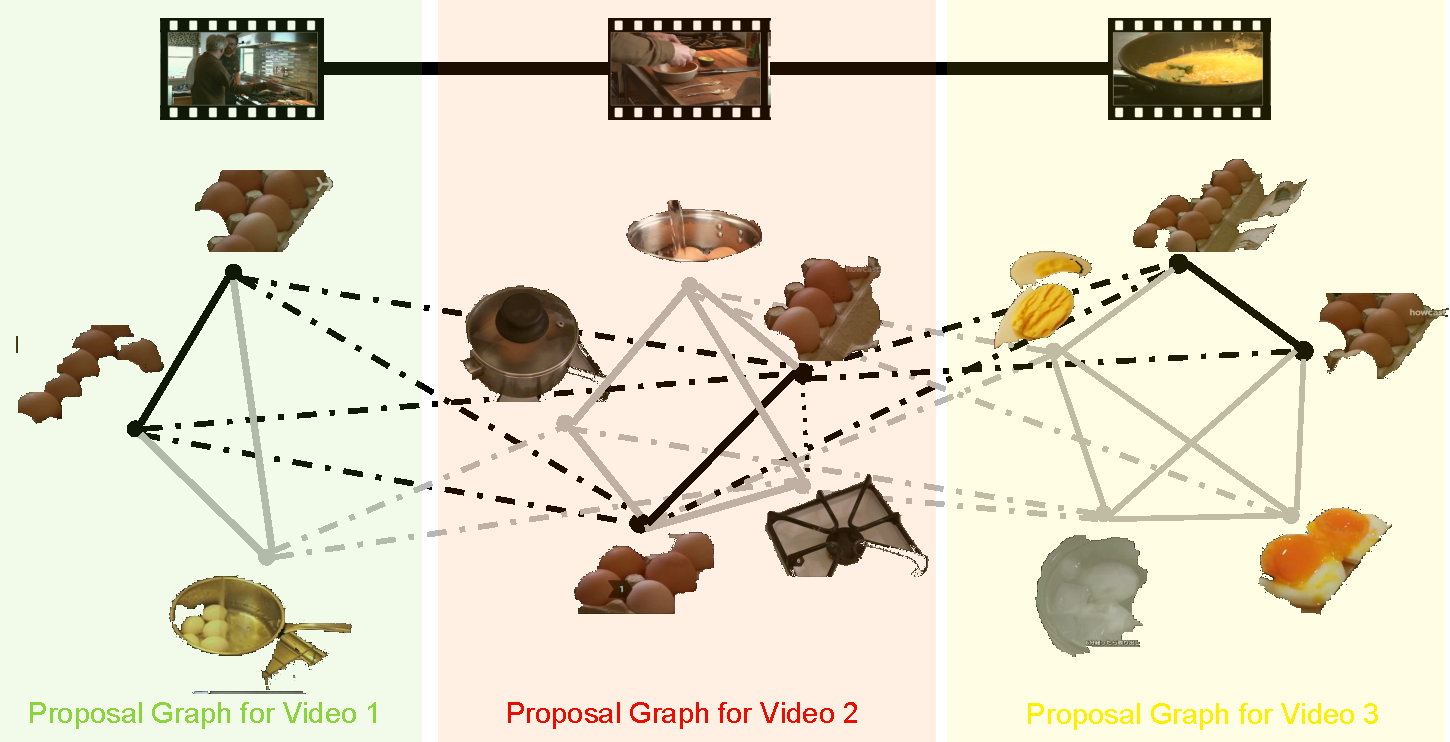
\includegraphics[width=0.48\textwidth]{joint_clustering}
  \scalebox{0.85}{$\arg\max  \color[HTML]{BF9000}{\frac{x_1^TA^{(1)}x^1}{x_1^Tx^1}}+\color[HTML]{990000}{\frac{x_2^TA^{(2)}x^2}{x_2^Tx^2}}+\color[HTML]{38761d}{\frac{x_3^TA^{(3)}x^3}{x_3^Tx^3}}+\color[HTML]{a64d79}{\frac{x_1^TA^{(1,2)}x^2}{x_1^T\mathds{1}\mathds{1}^Tx^2}}+\color[HTML]{F1C232}{\frac{x_2^TA^{(2,3)}x^3}{x_2^T\mathds{1}\mathds{1}^Tx^3}}$}
  \caption{\textbf{Visualization of the joint proposal clustering.} Here, we show the 1NN video graph and 2NN region graph. Each region proposal is linked to its 2 nearest neighbours from the video it belongs and 2 nearest neighbours from the videos it is neighbour of.}
  \label{hierProposal}
\end{figure}

We first explain the original spectral graph clustering algorithm and then extend it to joint clustering. Consider the set of region proposals extracted from a single video $r^k_t$, and a similarity metric $d(\cdot,\cdot)$ between any region proposal pair. We follow the single cluster graph partitioning (SCGP)\cite{scgp} approach to find the dominant cluster which maximizes the inter-cluster similarity. In other words, we solve
\begin{equation}
  \argmax_{x^k_t} \frac{\sum_{(k_1,t_1),(k_2,t_2) \in K \times T} x^{k_1}_{t_1} x^{k_2}_{t_2} d(r^{k_1}_{t_1},r^{k_2}_{t_2})}{\sum_{(k,t) \in K \times T} x^{k}_t}
\end{equation}
where, $x^{k}_t$ is a binary variable which is $1$ if $r^{k}_t$ is included in the cluster, $T$ is the number of frames and $K$ is the number of clusters per frame. When we use the vector form of the indicator variables as $\mathbf{x_{tK+k}}=x^{k}_{t}$ and the pairwise distance matrix as $\mathbf{A}_{t_1K+k_1,t_2K+k_2}=d(r^{k_1}_{t_1},r^{k_2}_{t_2})$, this equation can be compactly written as
$\argmax_{\mathbf{x}} \frac{\mathbf{x^T}A\mathbf{x}}{\mathbf{x^T}\mathbf{x}}$
Moreover, it can be solved by finding the dominant eigenvector of $\mathbf{x}$ after relaxing $x^{k}_t$ to $[0,1]$ \cite{scgp,scgp_eigen}. After finding the maximum, the remaining clusters can be found by removing the selected region proposals from the collection, and re-applying the same algorithm for the second dominant cluster.

Our extension of the SCGP into multiple videos is based on the assumption that the important objects of recipes occur in most of the videos. Hence, we re-formulate the problem by relating videos to each other. We use the kNN graph of the videos which we used for the outlier detection as explained in the Section~\ref{filter}. Moreover, we also create the kNN graph of region proposals in each video. This hierarchical graph structure is also visualized in Figure~\ref{hierProposal} for 3 videos. After creating this graph, we impose the similarity of regions in the selected cluster coming from each video as well as the similarity of regions coming from neighbour videos. Hence, given the pairwise distance matrices $\mathbf{A^{(i)}}$, binary indicator vectors $\mathbf{x^{(i)}}$ for each video and pairwise distance matrices for video pairs as $\mathbf{A^{(i,j)}}$, we define our optimization problem as;
\begin{equation}
\argmax \sum_{i \in N} \frac{\mathbf{x^{(i)^T}}\mathbf{A^{(i)}}\mathbf{x^{(i)}}}{\mathbf{x^{(i)^T}}\mathbf{x^{(i)}}} +
\sum_{i \in N} \sum_{j \in \mathcal{N}(i)} \frac{\mathbf{x^{(i)^T}}\mathbf{A^{(i,j)}}\mathbf{x^{(j)}}} {\mathbf{x^{(i)^T}}\mathds{1}\mathds{1}^T\mathbf{x^{(j)}}}
\end{equation}
where $\mathcal{N}(i)$ is the neighbours of the video $i$ in the kNN graph, $\mathds{1}$ is vector of ones and $N$ is the number of videos. We visualize this optimization objective in Figure~\ref{hierProposal} for the case of 3 videos.

After changing the optimization function, we can not use the efficient eigen-decomposition based approach from \cite{scgp,scgp_eigen}; however, we can use Stochastic Gradient Descent (SGD) since the cost function is quasi-convex when it is relaxed. We use the SGD with the following gradient function;
\begin{equation}
  \nabla_{\mathbf{x^{(i)}}} = \frac{2\mathbf{A^{(i)}} \mathbf{x^{(i)}} -2\mathbf{x^{(i)}} r^{(i)}}
  {\mathbf{{x^{(i)}}^T}\mathbf{x^{(i)}}}
+ \sum_{i \in N} \frac{\mathbf{A^{i,j}}\mathbf{x^{j}} - \mathbf{{x^{(j)}}^T} \mathds{1} r^{(i,j)}}{\mathbf{{x^{(i)}}^T} \mathds{1} \mathds{1}^T \mathbf{x^{(j)}} }
  %\text{Some vector matrix multiplication}
\end{equation}

where $r^{(i)}=\frac{\mathbf{x^{(i)^T}}\mathbf{A^{(i)}}\mathbf{x^{(i)}}}{\mathbf{x^{(i)^T}}\mathbf{x^{(i)}}}$ and $r^{(i,j)}=\frac{\mathbf{x^{(i)^T}}\mathbf{A^{(i,j)}}\mathbf{x^{(j)}}} {\mathbf{x^{(i)^T}}\mathds{1}\mathds{1}^T\mathbf{x^{(j)}}}$

After finding the dominant cluster by optimizing the cost function, we remove the selected cluster and re-apply the same algorithm to find the next dominant cluster. After finding $K=20$ clusters, we discard the remaining region proposals. In Figure~\ref{cvis}, we visualize some of the clusters which our algorithm generated after applied on the videos returned by the query \emph{How to Hard Boil an Egg}. As shown the figure, the resulting clusters are highly correlated and correspond to semantic objects\&concepts.
\begin{figure}[ht]
  \begin{subfigure}[b]{0.23\textwidth}
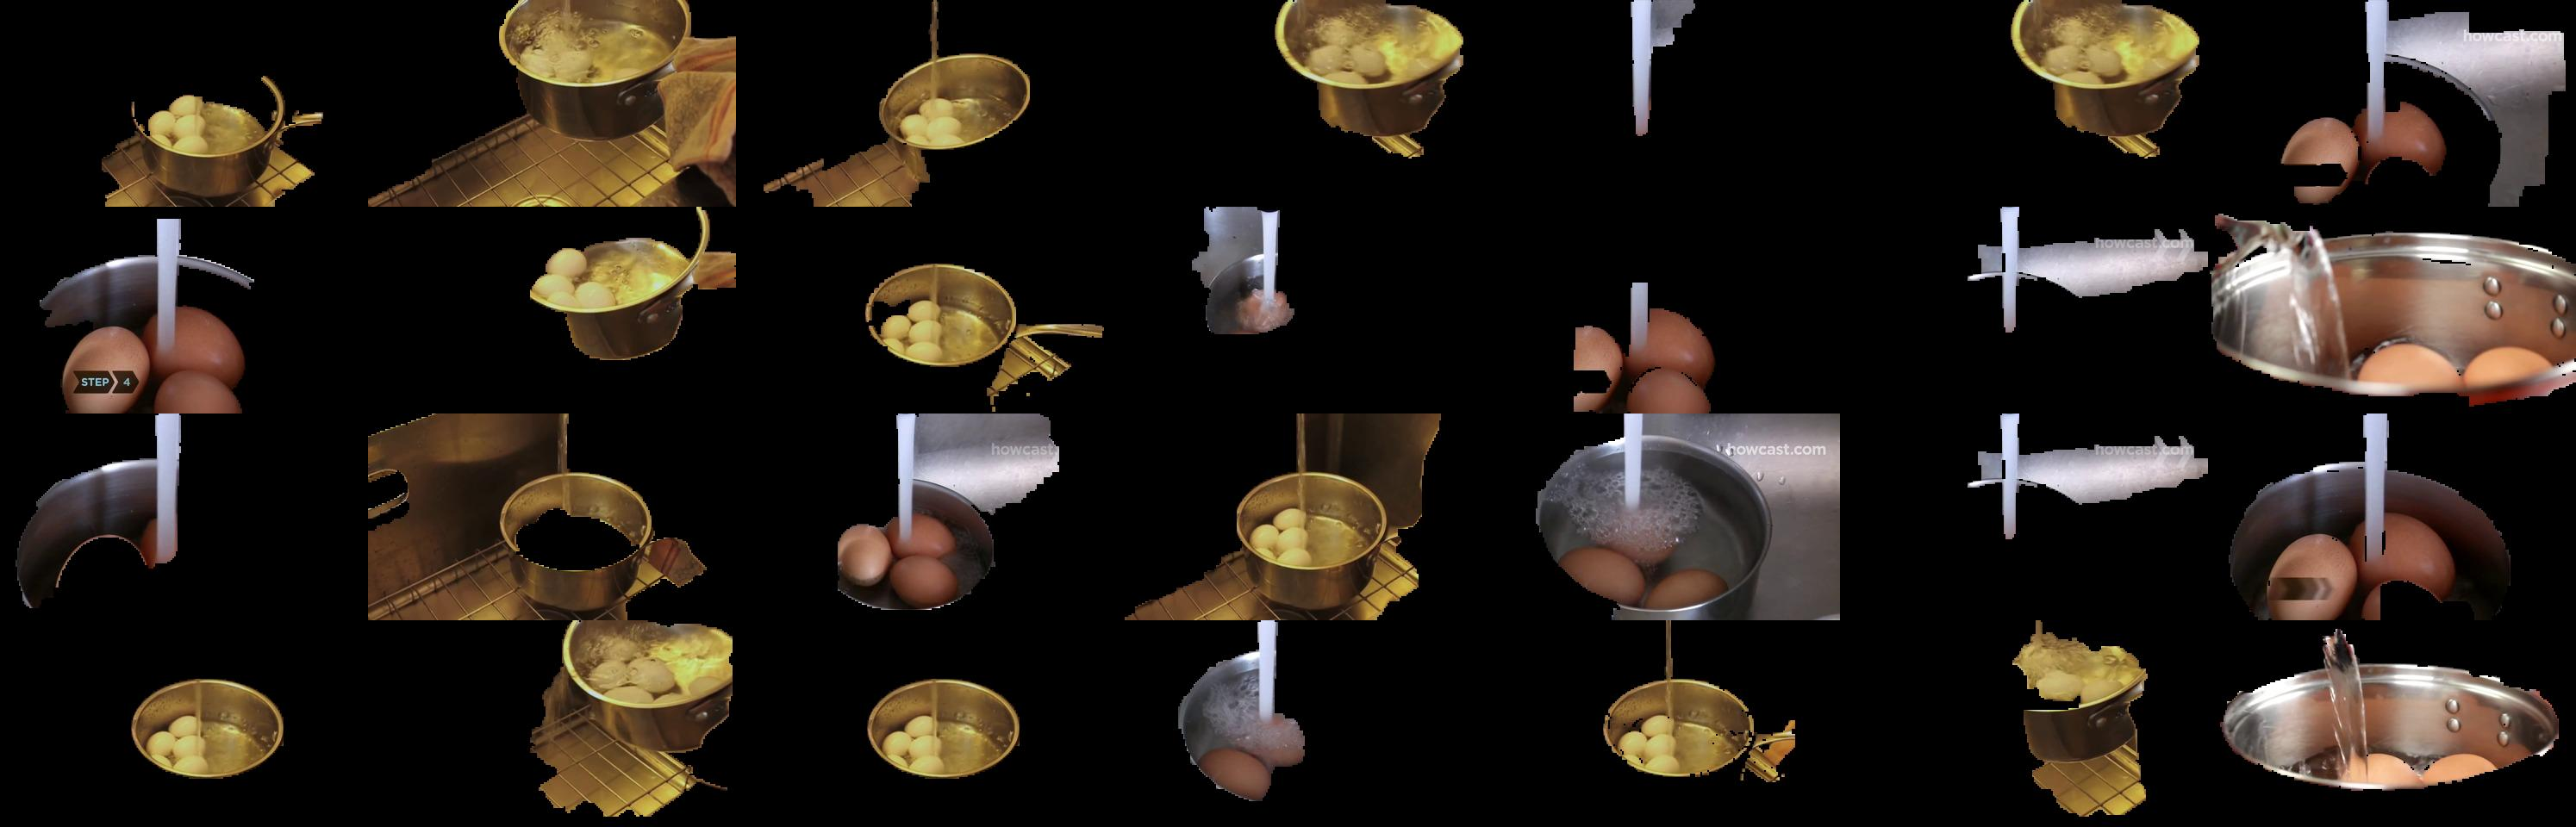
\includegraphics[width=\textwidth]{im0.png}
%\caption{Cluster 1}
\end{subfigure}
~
\begin{subfigure}[b]{0.23\textwidth}
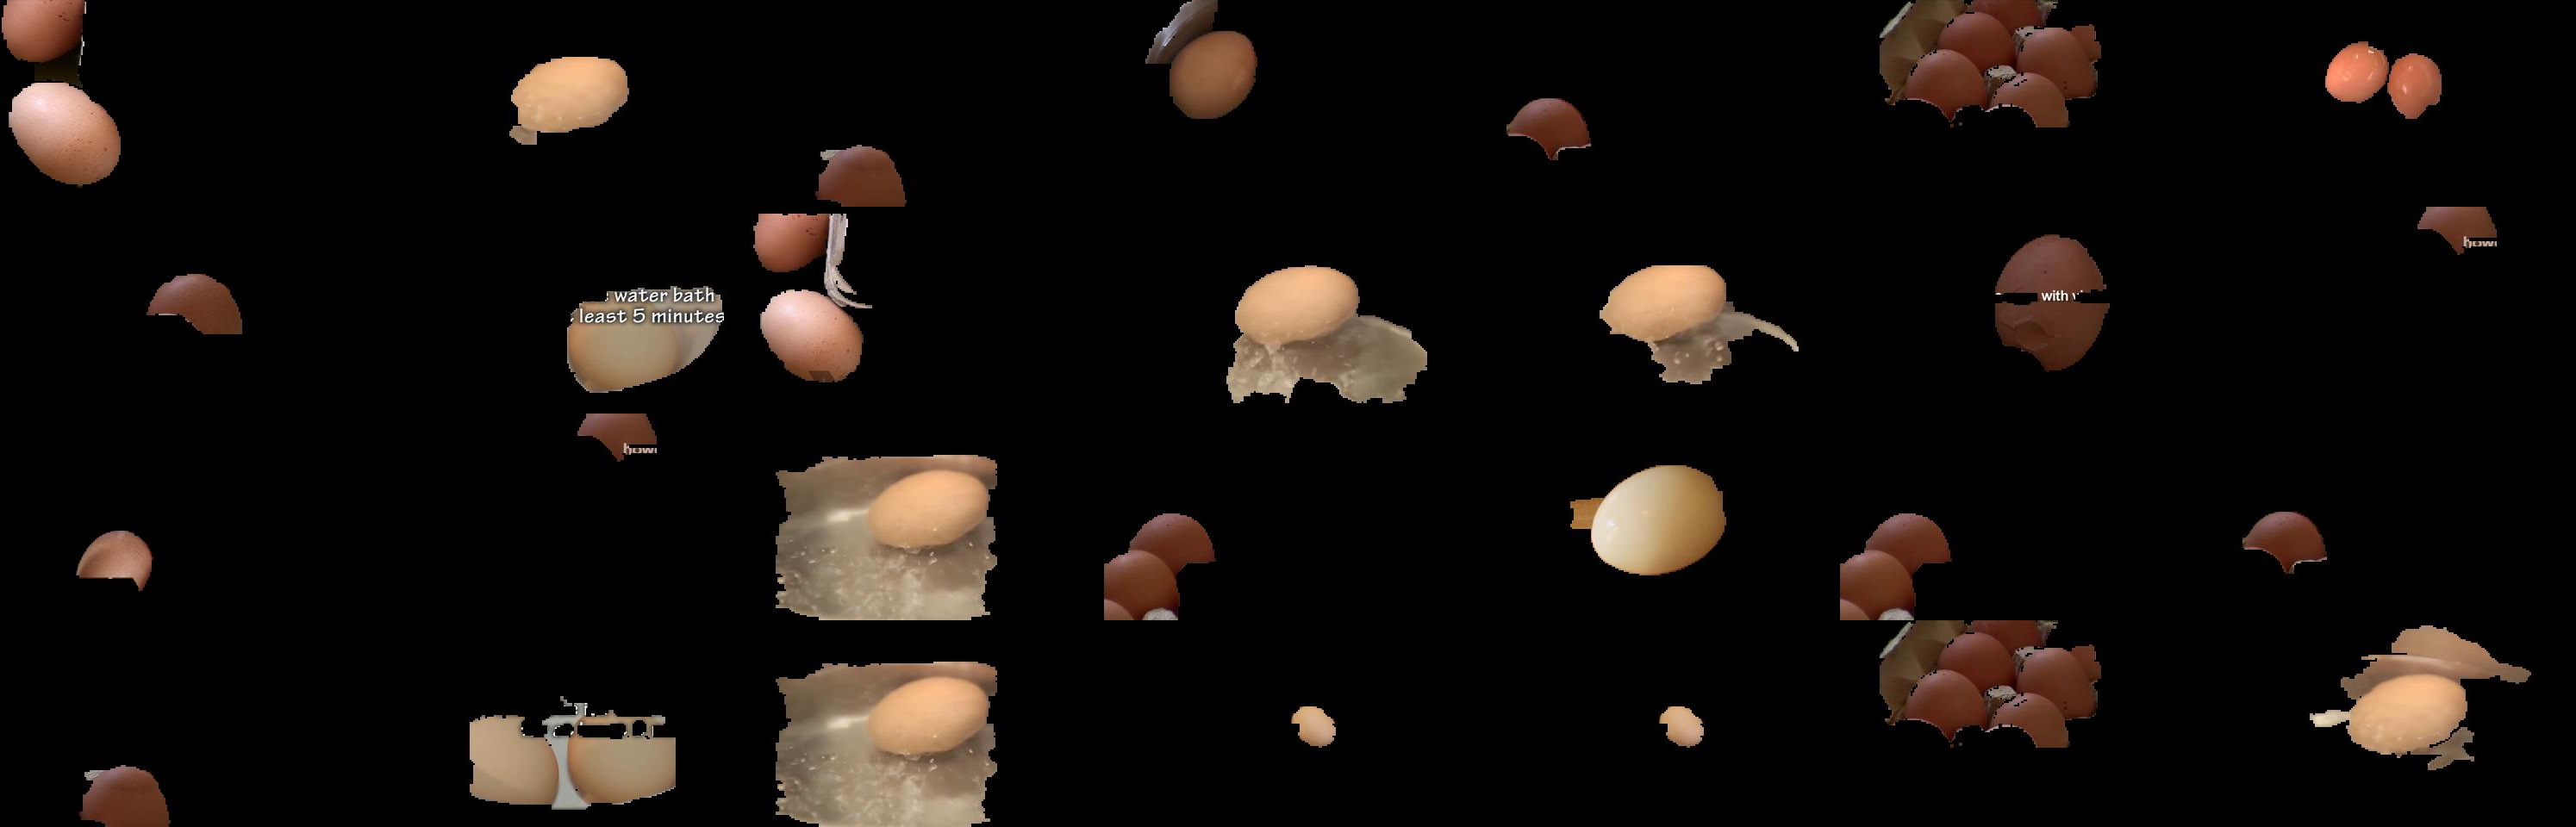
\includegraphics[width=\textwidth]{im4.png}
%\caption{Cluster 2}
\end{subfigure}
\begin{subfigure}[b]{0.23\textwidth}
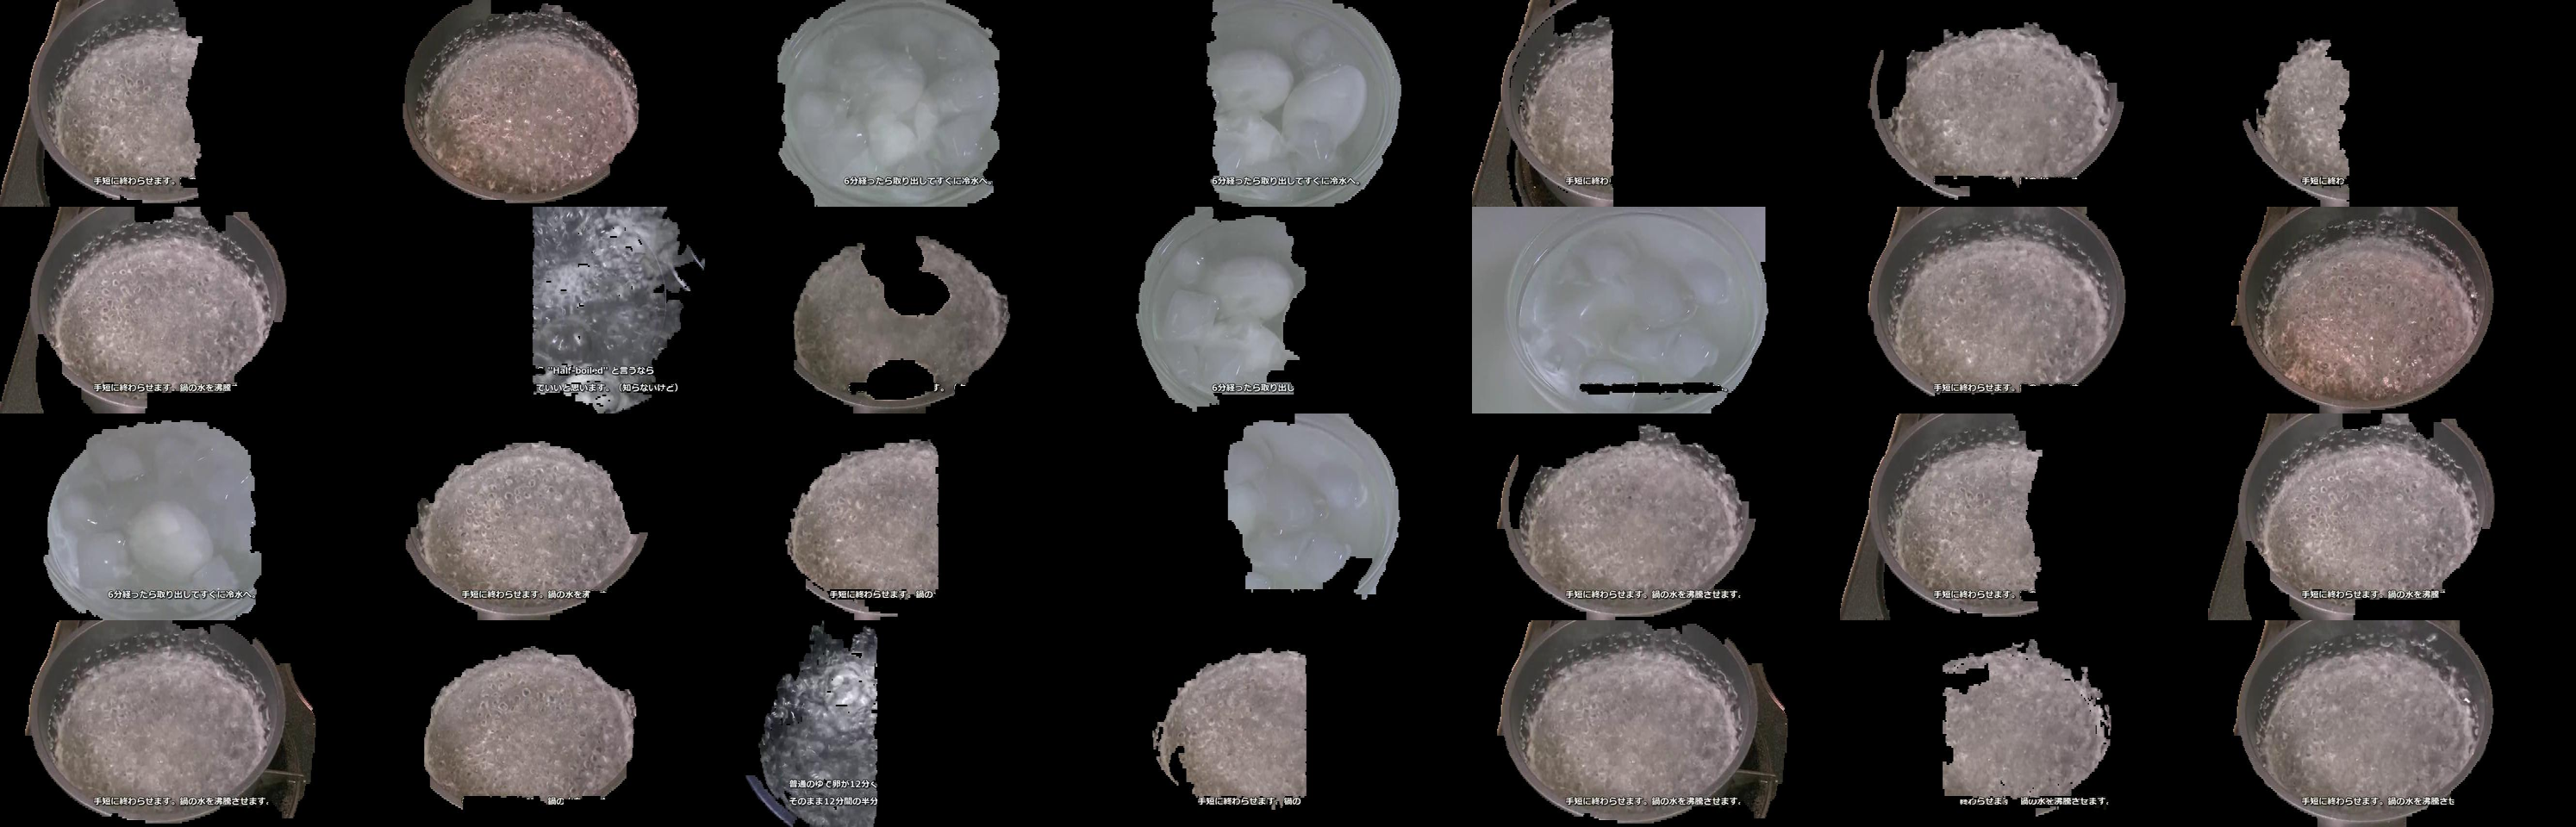
\includegraphics[width=\textwidth]{im5.png}
\end{subfigure}
~
\begin{subfigure}[b]{0.23\textwidth}
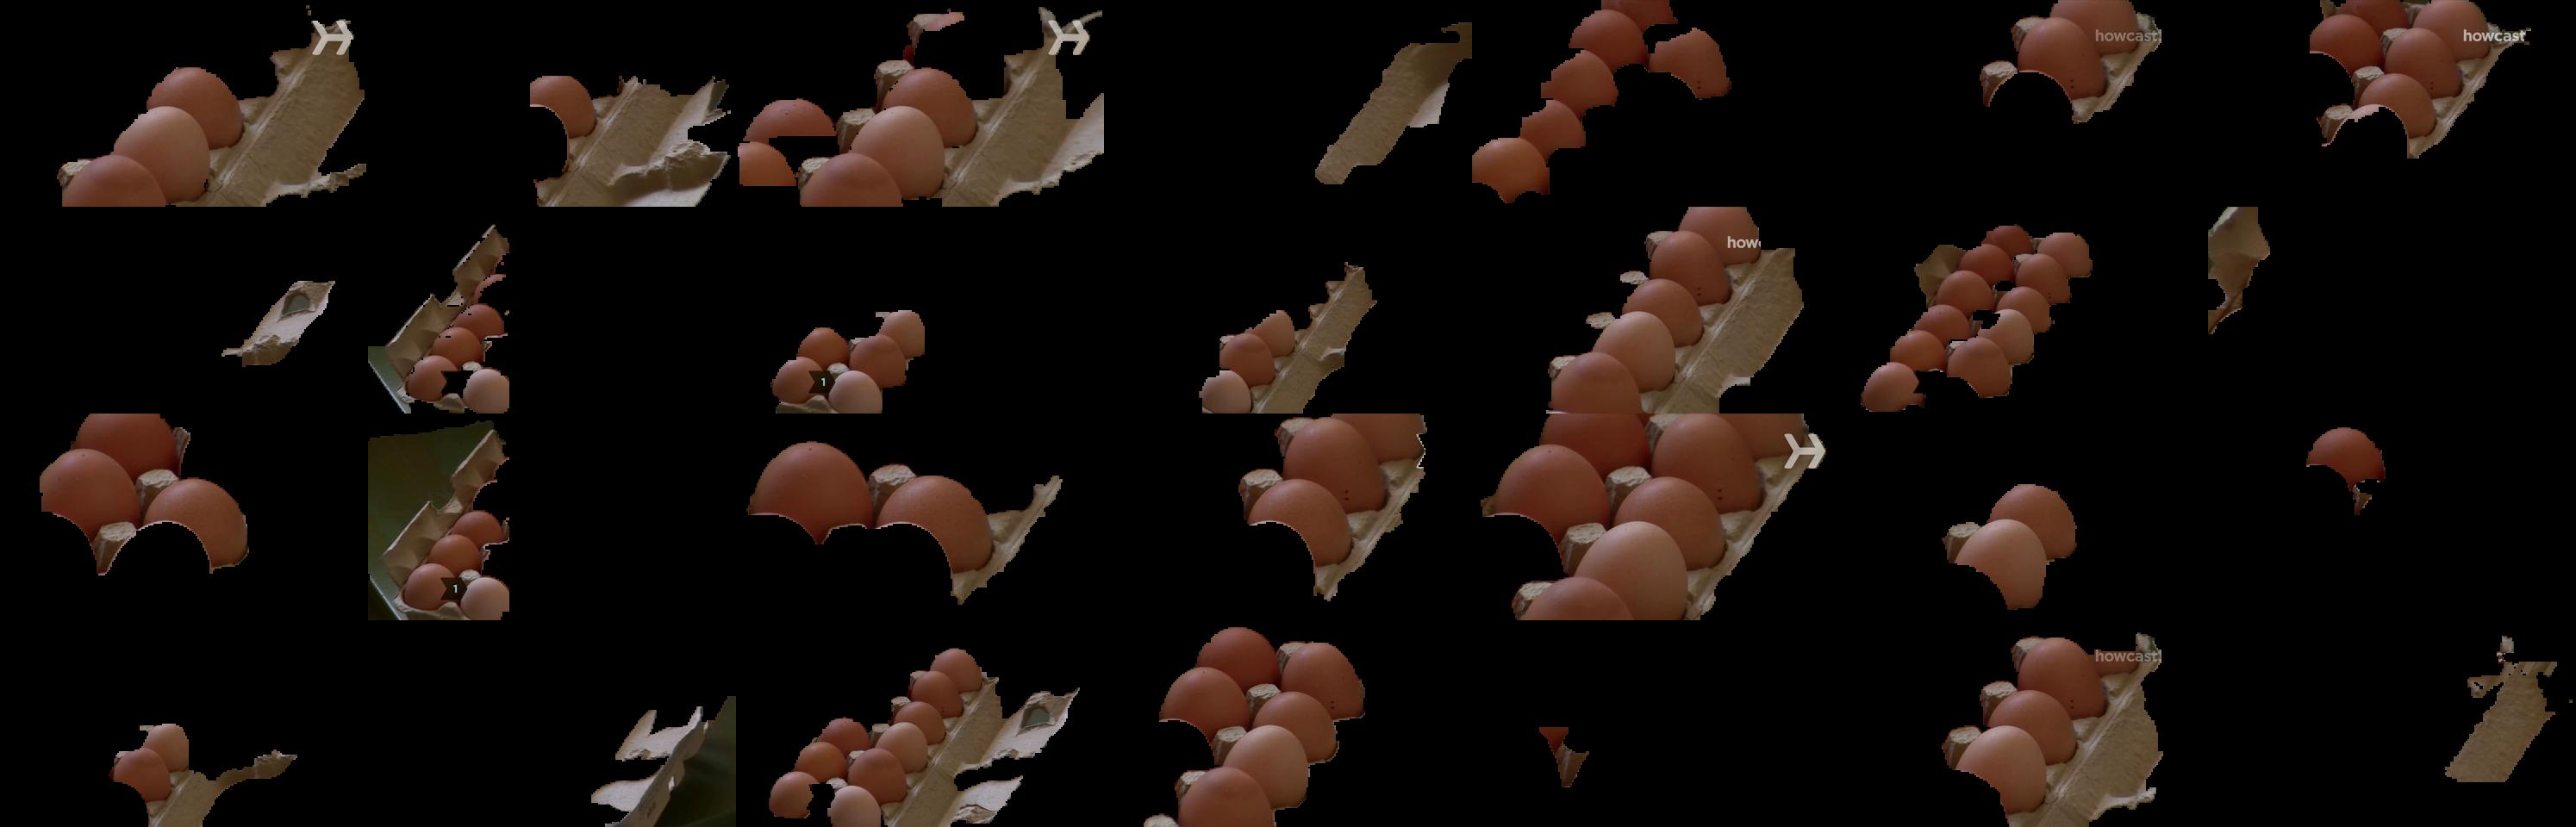
\includegraphics[width=\textwidth]{im7.png}
\end{subfigure}

\begin{subfigure}[b]{0.23\textwidth}
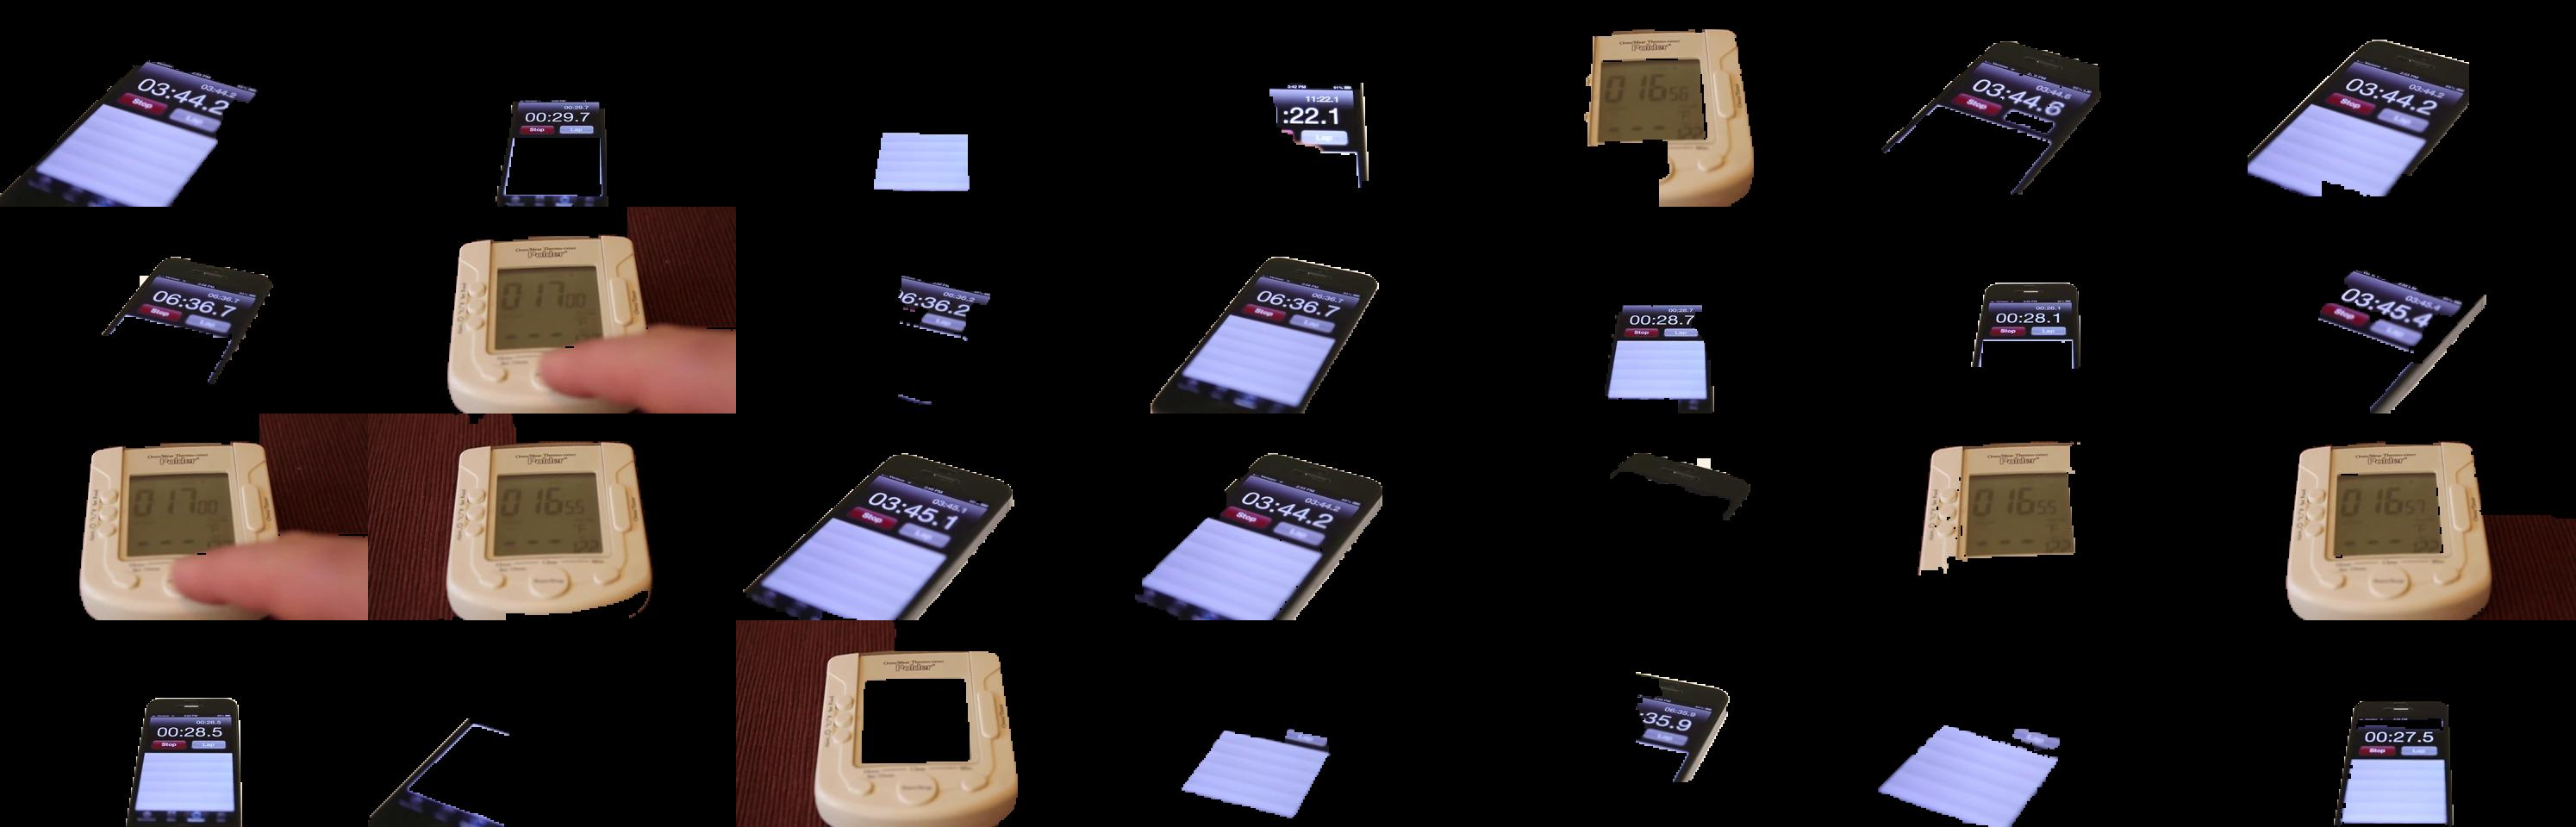
\includegraphics[width=\textwidth]{im8.png}
\end{subfigure}
~
\begin{subfigure}[b]{0.23\textwidth}
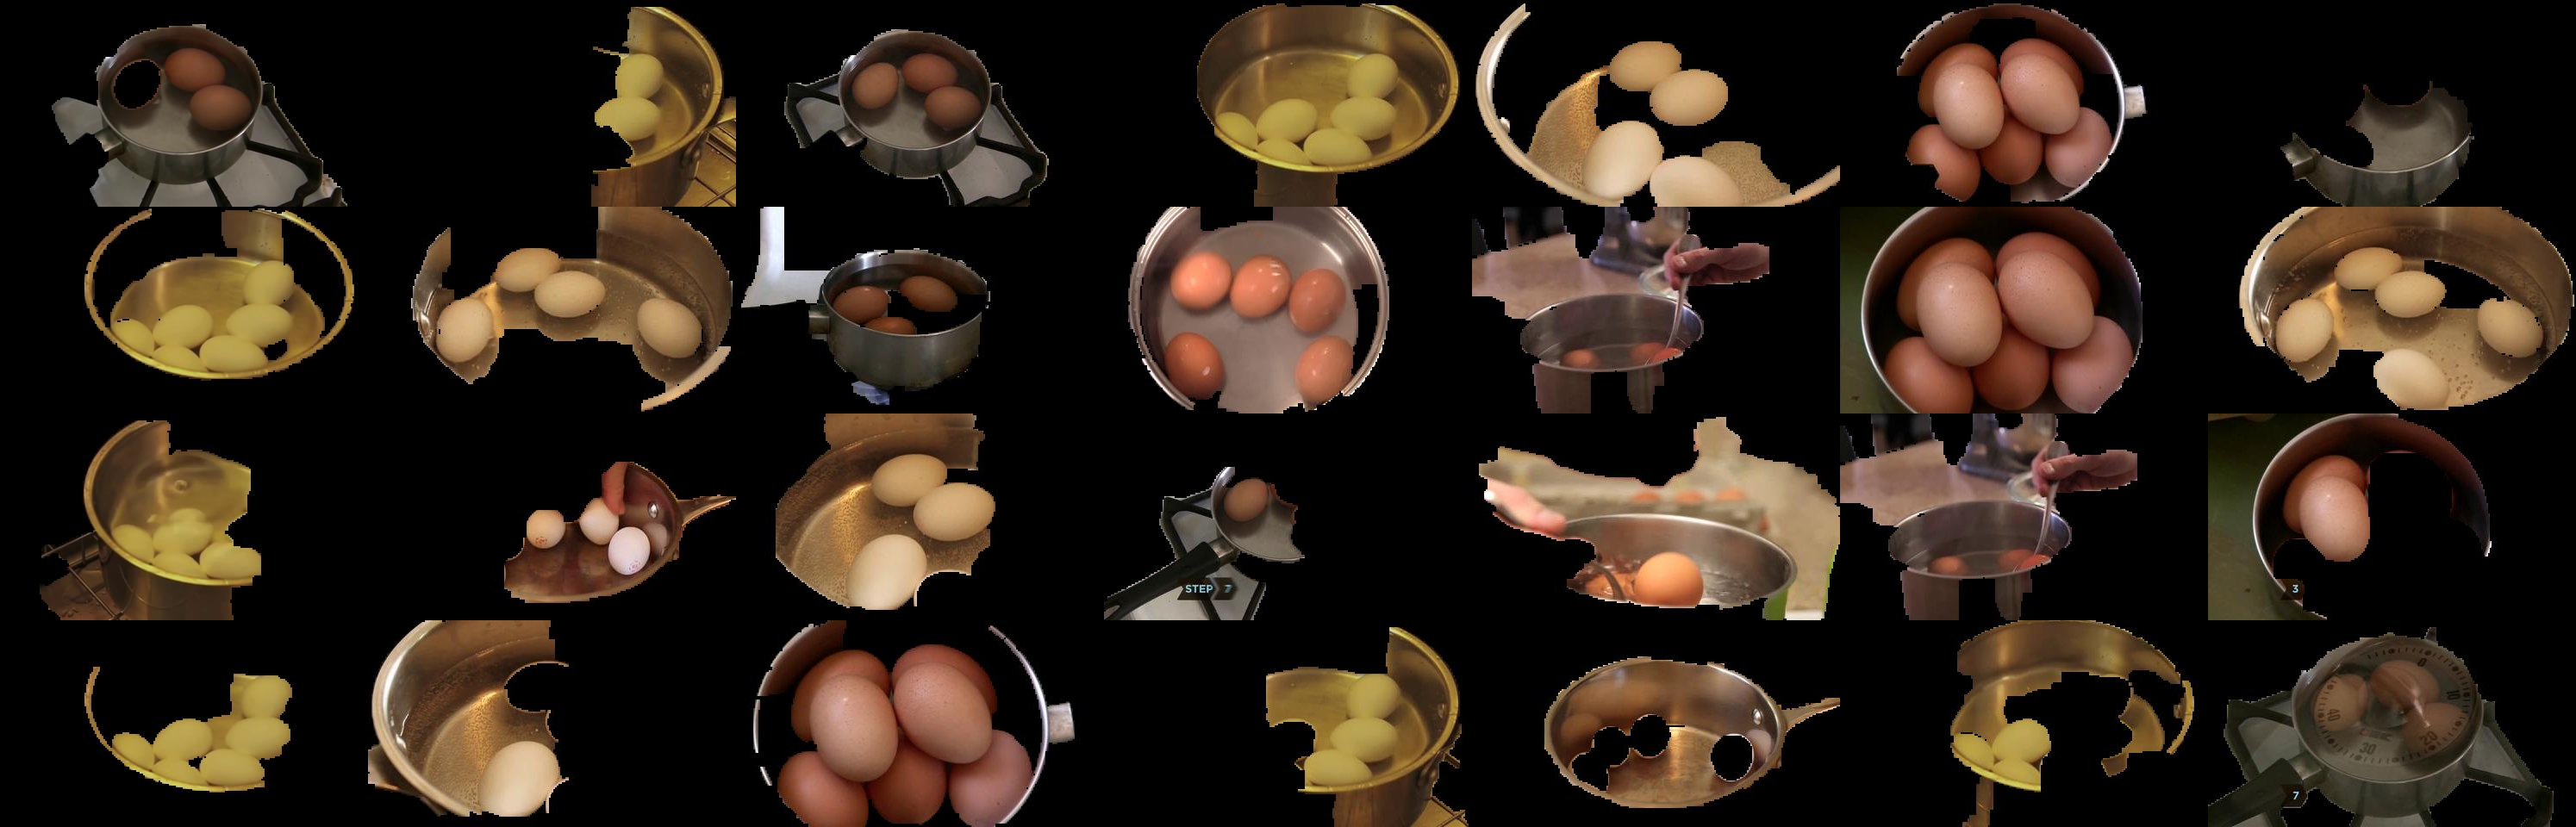
\includegraphics[width=\textwidth]{im10.png}
\end{subfigure}
\caption{Randomly selected images of randomly selected clusters learned for \emph{How to hard boil an egg?}}
\label{cvis}
\end{figure}


\subsubsection{Multi-Modal Representation of Frames}
After learning the objects and salient words, we represent each frame via the occurrence of salient words and objects. Formally, representation of the $t^{th}$ frame of the $i^{th}$ video is denoted as $\mathbf{y^{(i)}_t}$ and computed as $\mathbf{y^{(i)}_t}=[\mathbf{y^{(i),l}_t},\mathbf{y^{(i),v}_t}]$ such that $k^th$ entry of the $\mathbf{y^{(i),l}_t}$ is $1$ if the subtitle of the frame has the $k^{th}$ word and $0$ otherwise. $\mathbf{y^{(i),v}_t}$ is also a binary vector similarly defined over objects. We visualize the representation of a sample state in the Figure~\ref{visFrame}.

\begin{figure}
  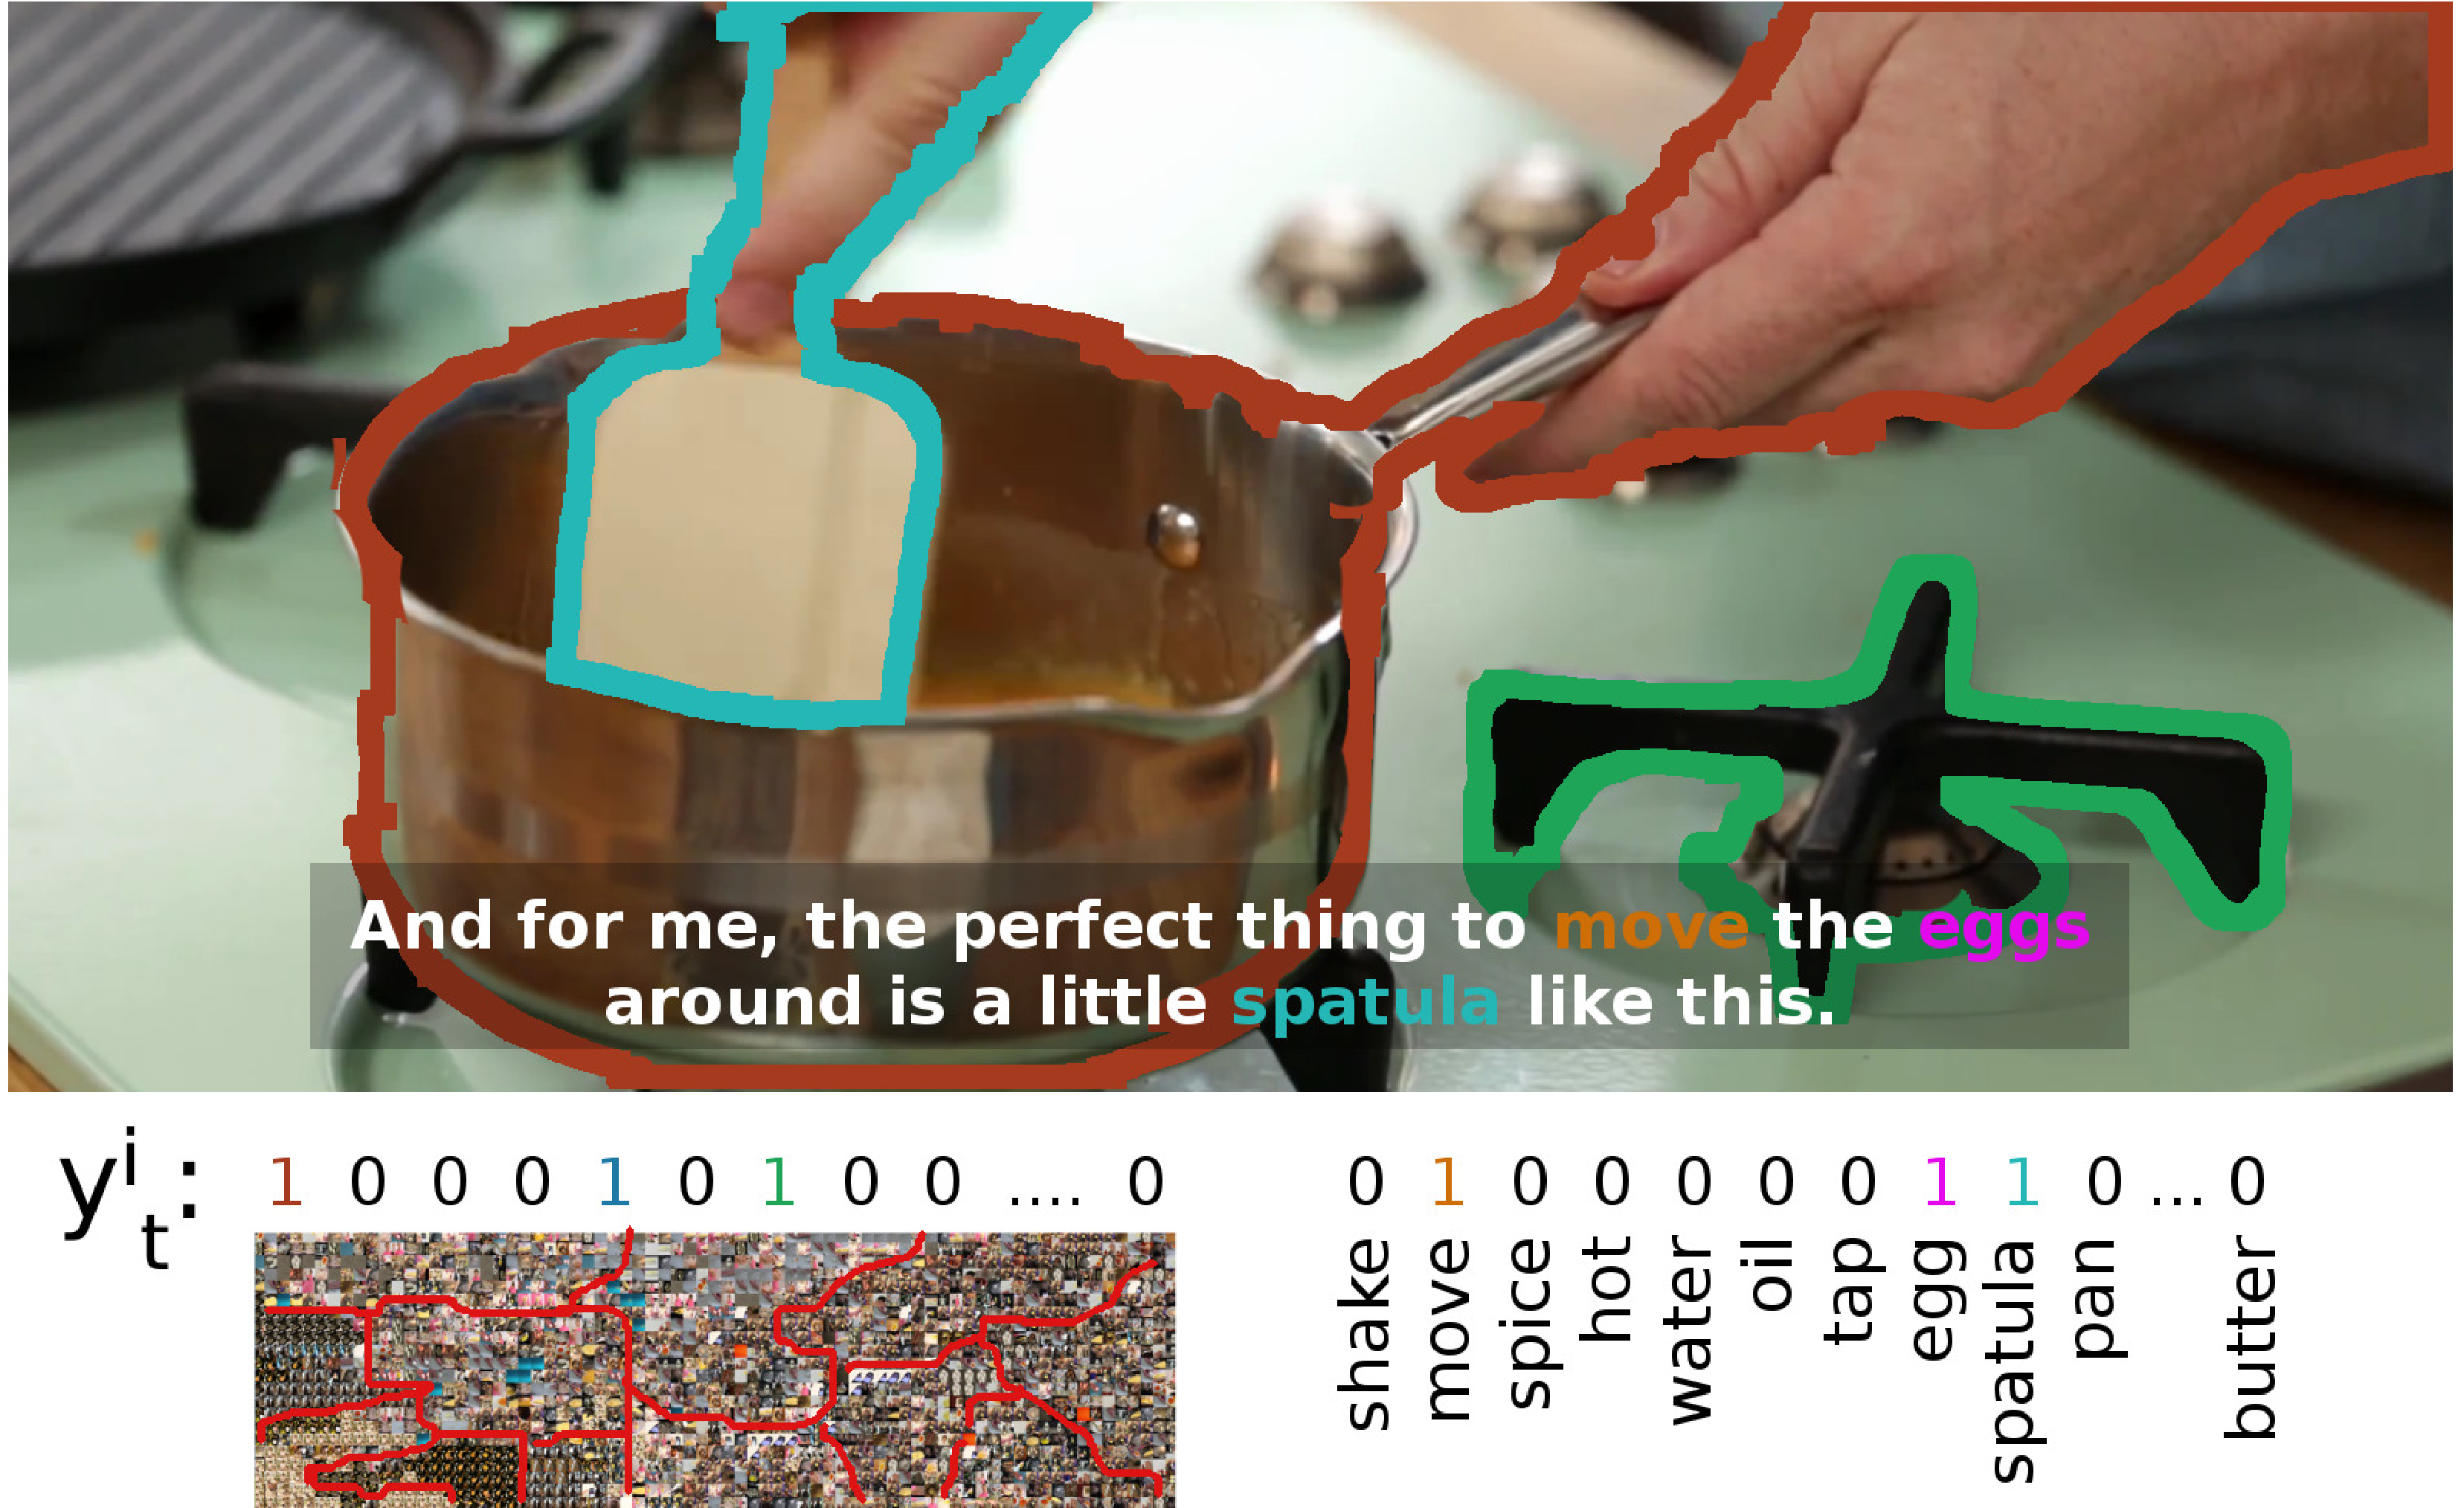
\includegraphics[width=0.48\textwidth]{frame}
  \caption{\textbf{Visualization of the representation of a sample frame.} 3 of the region proposals of the frame is included in the object clusters and 3 of the words in the subtitle of the frame is included in the salient word list.}
  \label{visFrame}
\end{figure}
